\documentclass[preprint,aps,prl,amsmath,amssymb,longbibliography]{revtex4-2}
\usepackage{graphicx}
\usepackage{dcolumn}
\usepackage{bm}
\usepackage{amsfonts}
\usepackage{xcolor,tabu}
\usepackage{multirow}
\usepackage{amsthm}
\usepackage{textcomp}
\usepackage{tikz}
\usepackage[colorlinks=true,
            linkcolor=blue,
            urlcolor=blue,
            citecolor=blue]{hyperref}
\hypersetup{bookmarksopen=true}
\usepackage{xr}


% \author{Zhengyang Liu, Wei Zeng, Xiaolei Ma, Xiang Cheng}
%\email{liux3141@umn.edu}
% \affiliation{Department of Chemical Engineering and Materials Science, University of Minnesota, Minneapolis, Minnesota 55455, USA}
\date{\today}

\begin{document}
\title{Giant Number Fluctuations and Energy Spectra\\
        in 3-D Bacterial Turbulence\\
        Supplemental Material}
\maketitle

% What is needed in this supplemental material?
% - all the methods I have used in the main text, including:
%   - bacterial samples
%   - microscopy
%   - GNF
%   - PIV
%   - cross-correlation
%   - energy spectra
% - Justification of methods and parameter choices
%   - two GNF methods
%   - local density flucution duration (10 frames)
% - Movie
%   - vigorous bacterial turbulence
%   - PIV overlay


\section{Materials and Methods}
\label{sec:method}
\subsection{Light-powered \textit{E. coli}}
We introduce a light-driven transmembrane proton pump, proteorhodopsin (PR), to wild-type \textit{E. coli} (BW25113) by transforming the bacteria with plasmid pZE-PR encoding the SAR86 $\gamma$-proteobacterial PR-variant (Walter 2007). The activity of PR is directly correlated with the light intensity. Thus, we can control the swimming speed of bacteria using light of different intensities.

The bacteria are cultured at 37 \textcelsius{} with a shaking speed at 250 rpm for 14-16 hours in terrific broth (TB) [tryptone 1.2\% (w/w), yeast extract 2.4\% (w/w), and glycerol 0.4\% (w/w)] supplemented with 0.1 g/L ampicillin. The culture is then diluted 1: 100 (v: v) in fresh TB and grown at 30 \textcelsius{} for 6.5 hours. PR expression is triggered by supplementing the culture medium with 1 mM isopropyl $\beta$-D-thiogalactoside and 10 \textmu M ethanolic all-trans-retinal in the mid-log phase (3 hours after the dilution).

The bacteria are harvested by gentle centrifugation (800g for 5 min). After discarding the culture medium in the supernatant, we resuspend bacteria with dI water. The resuspended suspension is then centrifuged again at 800g for 5 min, and finally adjusted to target concentration for microscopy.

\subsection{Sample preparation and microscopy}

To prepare the sample for microscopy, we put bacterial suspensions prepared from the previous step into a seal chamber made of glass slides (25 mm $\times$ 75 mm) and coverslips (18 mm $\times$ 18 mm). We first glue (NOA 81, Norland, NJ) two coverslips on a glass slide, side-by-side, leaving a 3-mm separation between the two coverslips. We then cover the 3-mm separation with another coverslip to form a ``channel''. Then we use pipet to inject bacterial suspensions into the channel. Finally, we seal the two ends of the channel using UV glue (NOA 76, Norland, NJ) to form a sealed chamber.

\subsection{Imaging and analysis}
\subsubsection{Microscopy}
Images of the bacterial suspensions are taken with a Nikon Ti-E inverted microscope using the bright field mode, and with a 20$\times$ (NA 0.5) objective. The field of view is 422 $\times$ 356 \textmu m$^2$. All videos are recorded at 30 frames per second using a sCMOS camera.
\subsubsection{Linear relation between intensity and density}
In the low attenuation limit (small thickness and weak absorptivity), $I=I_0-\epsilon$ where $\epsilon<<I_0$:
$$
\log \frac{I_0}{I} = \log \frac{I_0}{I_0 - \epsilon} \approx \frac{\epsilon}{I_0} \sim c
$$
$$
I = I_0 - \epsilon \sim c
$$
%%%%%%%%%%%%%%%%%%%%%%%%%%%%%%%%%%%%%%%%%%%%%%%%%%%%%%%%%%%%%%%%%%%%%%%%%%%%%%%%%%%%%%%%%%%
\subsection{Giant number fluctuations calculations}


The basic principle of measuring GNF is to get the scaling exponent of the standard deviation of the number of particles $\Delta N$ against the mean number $N$. We adopt the temporal variance \& spatial average (TVSA) method to do the calculation. Two different methods have been used in previous studies, and our choice will be justified later in Sec.~\ref{GNF-justification}.

The TVSA method starts by cropping square-shape subsystems of various sizes from the original image time series, as shown in Fig.~\ref{GNF-calculation}a. For each size $l$, a standard deviation $\Delta N$ and a mean $N$ are calculated over the time series. In order to add more statistics to the data extracted from a time series, we choose 20 evenly distributed spots (Fig.~\ref{GNF-calculation}b) as the seeds of the subsystems and average the results calculated from all these subsystems to give the result for a video. We vary the subsystem size $l$ from 10 \textmu m to 30 \textmu m, and examine the temporal variations (standard deviations) of bacterial concentrations $\Delta N_{ij}$ in the $i^{th}$ frame for each box size $l_j$. The temporal variations are then averaged in space (over $i$) to give a single value variation $\Delta N_{j}$.
Then number fluctuations in the system is captured by the dependence of $\Delta N_{j}$ on $l_j$. In an equilibrium system, $\Delta N_{j}\propto l_j$ (this follows from $\Delta N_{j}\propto \sqrt{N_j}$ and $N_j\propto l_j^2$).
Thus, the deviation from $\Delta N_{j}\propto l_j$ quantifies the giant number fluctuation in the system.
In the main paper, we plot $\Delta N_{j}/l_j$ as a function of $l_j^2/l_b^2$, where $l_b$ is the length scale of single bacterial body length, chosen to be 3 \textmu m.
To be consistent with the notations in literatures, we get rid of the subscript $j$, and write $l_j$ as $\sqrt{N}$.
Note that the subscript $j$ denotes different choices of box sizes.

Without a more careful calibration, we are not able to obtain the exact number of particles using this Beer's law based method. Fortunately, the calculations of GNF does not require the exact number, but only the relative number. In the main paper, we show that the volume fractions $\phi$ and average pixel intensities $I$ follow a pretty linear relation. Such a relation entails that $\Delta I \propto \Delta N$, which is followed by $\Delta I/\sqrt N \propto \Delta N/\sqrt N$. The proportionality allows us to get the scaling exponents of $\Delta N/\sqrt N$ against $N$, without having to measure the exact particle numbers.

\begin{figure}[!]
\begin{center}
\includegraphics[width=0.8\textwidth]{figures/GNF-calculation/v1.pdf}
\caption[Concentration dependence of GNF.]
{
\textbf{GNF calculations.}
(a) Varying subsystem sizes.
(b) Multiple seeds of subsystems for spatial average.
}
\label{GNF-calculation}
\end{center}
\end{figure}


\subsection{Particle image velocimetry (PIV)}

The flow fields are measured by Particle Image Velocimetry (PIV) analysis using openPIV package in Python %(Fig.~\ref{fig:1}b).
We choose box size to be 16 \textmu m, which is much larger than a single bacterium body to enhance statistical accuracy, and smaller than the typical length scale of the collective motion of \textit{E. coli} so that the features are not smoothed out. We choose step size to be half of the box size (8 \textmu m) by convention.

\subsection{Cross correlation}

The cross correlation calculation used when analyzing the local correlation between kinetic energy and density fluctuations is defined as the following:
\begin{equation}
\label{eq:cross-correlation}
A\star B = \frac{\langle(A-\bar A)(B-\bar B)\rangle}{\sigma_A\sigma_B}
\end{equation}
where $A$ and $B$ are two arrays of scalars, $\star$ is the operator standing for cross correlation, $\bar\cdot$ means taking the mean, $\sigma$ means the standard deviation, and $\langle\cdot\rangle$ denotes taking the average of all scalars in an array. The cross correlation quantifies the similarity between arrays $A$ and $B$. The resulting number takes value from -1 to 1.

\subsection{Energy spectra}
We calculate the energy spectra using the following formula
\begin{equation}
E(k_x, k_y) = \frac{\langle u_k(k_x, k_y)u^*_k(k_x, k_y)+v_k(k_x, k_y)v_k^*(k_x, k_y)\rangle}{2A}
\end{equation}
where $E$ is the energy density in $k$ space, $u_k$ and $v_k$ are $k$ space velocity fields, $A$ is the real space area of the system and $^*$ denotes the complex conjugate. The $\langle\cdot\rangle$ denotes an average over multiple images from different times. This method can be shown to be equivalent to another commonly used formula, which calculates the Fourier transform of real space velocity spatial correlation functions:
\begin{equation}
E^1 = \int \langle \boldsymbol{u}(\boldsymbol{r_0}) \boldsymbol{u}(\boldsymbol{r_0}+\boldsymbol{r}) \rangle
        e^{-i\boldsymbol{k}\cdot\boldsymbol{r}} d\boldsymbol{r}
\end{equation}

We show here how they are equivalent by considering one of the velocity componenet $u$. Starting with the definition of $E$
\begin{equation}
\begin{split}
E(k_x, k_y) &= u_k(k_x, k_y)u_k^*(k_x, k_y)\\
& = \iint u(x, y)e^{-ik_xx}e^{-k_yy}dxdy\left[\iint u(x', y')e^{-ik_xx'}e^{-ik_yy'}dx'dy'\right]^*\\
& = \iint u(x, y)e^{-ik_xx}e^{-k_yy}dxdy\iint u^*(x', y')e^{ik_xx'}e^{ik_yy'}dx'dy'\\
& = \iiiint u(x, y)u(x', y')e^{-ik_x(x-x')}e^{-k_y(y-y')}dxdydx'dy'
\end{split}
\end{equation}
here, we change variable and let $x'' = x - x'$ and $y'' = y - y'$ the original expression can be rearranged into
\begin{equation}
\begin{split}
& \iiiint u(x'+x'', y'+y'')u(x', y')e^{-ik_xx''}e^{-k_yy''}d(x'+x'')d(y'+y'')dx'dy'\\
& = \iint \left[\iint u(x'+x'', y'+y'')u(x', y')dx'dy'\right] e^{-ik_xx''}e^{-k_yy''} d(x'+x'')d(y'+y'')
\end{split}
\end{equation}
using the definition of velocity correlation function (average all possible pairs over available space):
\begin{equation}
\langle u(x, y)u(x+x'', y+y'') \rangle = \frac{\iint u(x'+x'', y'+y'')u(x', y')dx'dy'}{\iint dx'dy'}
\end{equation}
we obtain
\begin{equation}
\iint dx'dy'\iint \langle u(x, y)u(x+x'', y+y'') \rangle e^{-ik_xx''}e^{-k_yy''} dx''dy''
\end{equation}
the first integration is the available space size of velocity field, in this case the system area $A$. Thus,
\begin{equation}
E(k_x, k_y) = E^1(k_x, k_y)
\end{equation}



\section{Justification of methods and parameter choices}
\label{GNF-justification}
\subsection{Two methods for calculating GNF}


Two methods have been used to quantify giant number fluctuations. Both divide the whole system into many small subsystems. Then, one of them calculates the mean number $N$ and standard deviation $\Delta N$ over time, and then average spatially (temporal variance -> spatial average, TVSA) \cite{Narayan2007}. The other calculates $N$ and $\Delta N$ over all the small subsystems in one frame, then takes an average over time (spatial variance -> temporal average, SVTA) \cite{Aranson2008}.

Urbach 2008 futher stated that when a system is homogeneous, where spatial and temporal correlations are small compared with the system size and experiment duration, two methods give the same result. Our experimental system, \textit{E. coli} suspensions, has a correlation length ($\sim 30$ \textmu m) much smaller than the system size ($\sim 140$ \textmu m), and is thus a spatially homogeneous system. If observed over a sufficiently long time (longer than the autocorrelation time), the system can be regarded as being temporally homogeneous as well.

In real experiment, we rely on image pixel intensity to measure local concentrations. The illumination light in our microscope system, and probably all microscope systems, presents a slight inhomogeneity which is quite stable and long-standing. This has caused trouble when we tried to use the second method (SVTA) to measure GNF (show a figure of GNF in stationary samples). In principle, such inhomogeneity can be removed by a removing the background preprocessing. However, without enough images for a sample, such a preprocessing may lead to larger errors. As a result, we adopt the TVSA method, which is not sensitive to the long-standing spatial inhomogeneity and works more robustly in our measurement. A way to understand the fact that TVSA is not sensitive to illumination inhomogeneity is to think of it as adding a constant image to each frame, which does not affect the temporal variation calculation.

\subsection{Video length for calculating local density fluctuations}
When calculating the local density fluctuations, we want to measure the instantaneously change of density instead of a steady-state scaling. Thus, we choose the length of video for this calculation to be within the autocorrelation time of density (or more accurately, average pixel intensity) variations. We also want to include as many frames as we can instead of using adjacent frame, in order to suppress the effects from random fluctuations of image intensities, the nature of optical imaging.

We first calculate the autocorrelation functions of density. The basic principle of this calculation is to shift a time series of density at varying steps and calculate the matching between the original series and the shifted series, using the cross correlation scheme as in Eq.~\ref{eq:cross-correlation}. In Fig.~\ref{density-autocorrelation}, we plot the autocorrelation function of density at various volume fractions, covering the range studied in this work. We notice that low volume fraction suspensions display a longer correlation time. The smallest correlation time, according to this measurement, is around 1 second, which corresponds to 30 frames in our videos. Thus, we choose 10 frames as the video length for calculating the local density fluctuations, which is much smaller than the correlation time but still has many enough frames to suppress the random flucutations from imaging.


\begin{figure}[!]
\begin{center}
\includegraphics[width=0.7\textwidth]{figures/density-autocorrelation/v1.pdf}
\caption[Density autocorrelation]
{
\textbf{Density autocorrelation.}
}
\label{density-autocorrelation}
\end{center}
\end{figure}



\bibliographystyle{apsrev4-2}
\bibliography{../correlation}




\end{document}


\end{document}
